\documentclass[12pt]{article}
\usepackage{tikz}
\usetikzlibrary{trees, positioning, shapes}
\usepackage{amsmath}
\usepackage{algorithm}
\usepackage{algpseudocode}

\begin{document}

\title{Monte Carlo Tree Search (MCTS) for HEX Step-by-Step Visualization}
\author{Christophe Louargant}
\date{\today}
\maketitle

\section*{MCTS Algorithm Overview}

The MCTS algorithm consists of four phases repeated for many iterations:

\begin{enumerate}
    \item \textbf{Selection}: Traverse the tree from root to leaf using UCB1
    \item \textbf{Expansion}: \it{the name is somehow confusing}
    \begin{itemize}
    \item \textit{Initial Phase}: Add new child to root (tree grows wider) 
    \item \textit{Subsequent Phases}: Reuse existing child (no growth)
    \end{itemize}
    \item \textbf{Simulation}: Run random playout from the new node
    \item \textbf{Backpropagation}: Update statistics along the path
\end{enumerate}

\section*{UCB1 Formula}

\[
\text{UCB1}(i) = \frac{w_i}{n_i} + c \sqrt{\frac{\ln N}{n_i}}
\]

Where:
\begin{itemize}
    \item $w_i$: Number of wins for node $i$
    \item $n_i$: Number of visits for node $i$  
    \item $N$: Total number of visits to parent node
    \item $c$: Exploration constant (typically $\sqrt{2}$)
\end{itemize}

\section*{Step-by-Step Visualization}

Suppose the board is in a state
(represented by the root node of the tree) where there
remains 5 positions available on the board for
the current player (MCTS engine) to choose.


\subsection*{Initial State}
Root node with 5 available moves: 
$A_1, A_2, A_3, A_4, A_5$. All unvisited.

\begin{center}
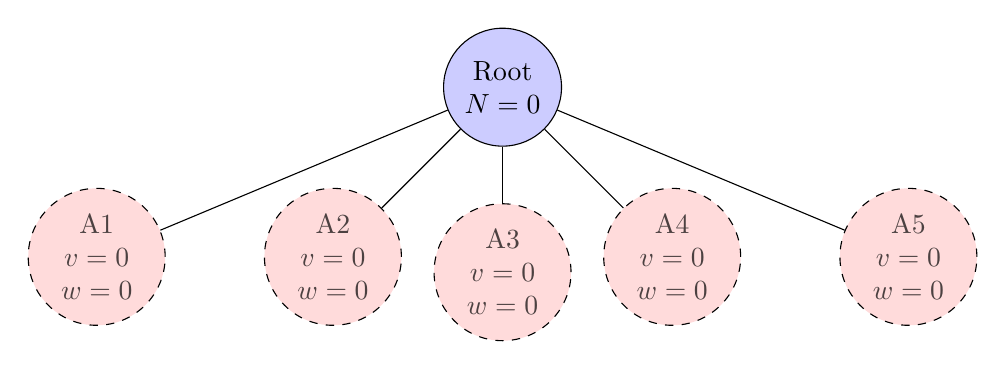
\begin{tikzpicture}[
    node distance=2.35cm,
    treenode/.style={circle, draw, minimum size=1cm, align=center},
    root/.style={treenode, fill=blue!20},
    unvisited/.style={treenode, fill=red!20,
        fill opacity=0.7, % Adjust transparency (0.0 to 1.0)
        draw,              % Ensure a border is drawn
        dashed             % Make the border dashed
        },
    visited/.style={treenode, fill=green!20},
    simulation/.style={rectangle, draw, dashed, fill=yellow!20}
]

% Root node
\node[root] (root) {Root\\$N=0$};

% Available moves (unvisited)
\node[unvisited, below left=1cm and 4cm of root] (a1) {A1 \\ $v=0$ \\ $w=0$};
\node[unvisited, below left=1cm and 1cm of root] (a2) {A2 \\ $v=0$ \\ $w=0$};
\node[unvisited, below of=root] (a3) {A3 \\ $v=0$ \\ $w=0$};
\node[unvisited, below right=1cm and 1cm of root] (a4) {A4 \\ $v=0$ \\ $w=0$};
\node[unvisited, below right=1cm and 4cm of root] (a5) {A5 \\ $v=0$ \\ $w=0$};

% Edges
\draw (root) -- (a1);
\draw (root) -- (a2);
\draw (root) -- (a3);
\draw (root) -- (a4);
\draw (root) -- (a5);

\end{tikzpicture}
\end{center}

\subsection*{Iteration 1: First Expansion}

All nodes have UCB1 = $\infty$ (division by zero). Randomly select A1.

\begin{center}
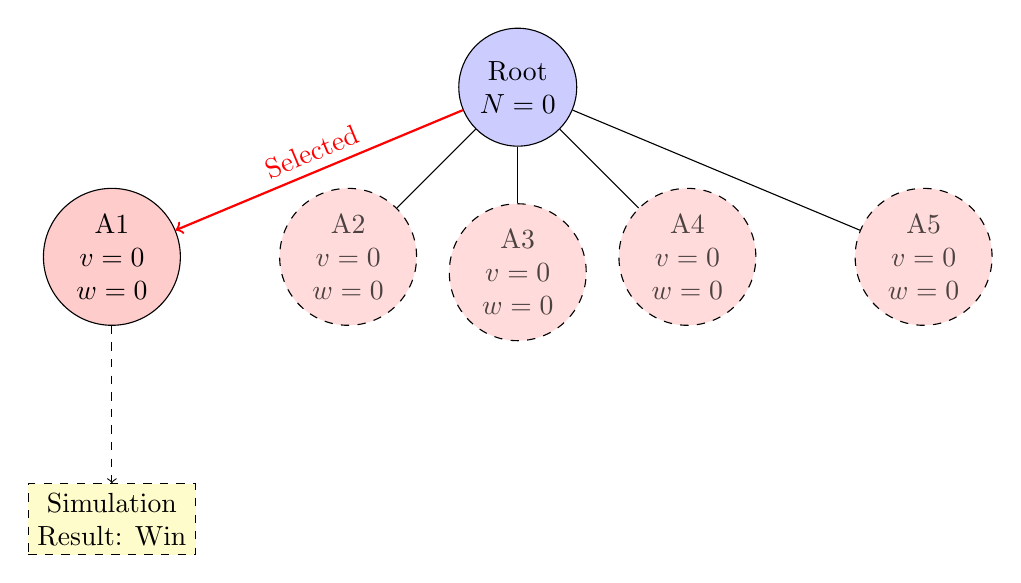
\begin{tikzpicture}[
    node distance=2.35cm,
    treenode/.style={circle, draw, minimum size=1cm, align=center},
    root/.style={treenode, fill=blue!20},
        unvisited/.style={treenode, fill=red!20,
        fill opacity=0.7, % Adjust transparency (0.0 to 1.0)
        draw,              % Ensure a border is drawn
        dashed             % Make the border dashed
        },
    selected/.style={treenode, fill=red!20},
    visited/.style={treenode, fill=green!20},
    simulation/.style={rectangle, draw, dashed, fill=yellow!20, align=center}
]

% Root node
\node[root] (root) {Root \\ $N=0$};

% A1 is being expanded (selected)
\node[selected, below left=1cm and 4cm of root] (a1) {A1 \\ $v=0$ \\ $w=0$};
\node[unvisited, below left=1cm and 1cm of root] (a2) {A2 \\ $v=0$ \\ $w=0$};
\node[unvisited, below of=root] (a3) {A3 \\ $v=0$ \\ $w=0$};
\node[unvisited, below right=1cm and 1cm of root] (a4) {A4 \\ $v=0$ \\ $w=0$};
\node[unvisited, below right=1cm and 4cm of root] (a5) {A5 \\ $v=0$ \\ $w=0$};

% Simulation cluster
\node[simulation, below=2cm of a1] (sim1) {Simulation \\ Result: Win};

% Edges and annotations
\draw[->, thick, red] (root) -- node[above, sloped] {Selected} (a1);
\draw (root) -- (a2);
\draw (root) -- (a3);
\draw (root) -- (a4);
\draw (root) -- (a5);
\draw[dashed, ->] (a1) -- (sim1);

\end{tikzpicture}
\end{center}

\textbf{Backpropagation}: $A_1$ wins $\Rightarrow$ $v=1$, $w=1$, Root $N=1$

\subsection*{Iteration 2: Second Expansion}

Unvisited nodes still have UCB1 = $\infty$. Randomly select A2.

\begin{center}
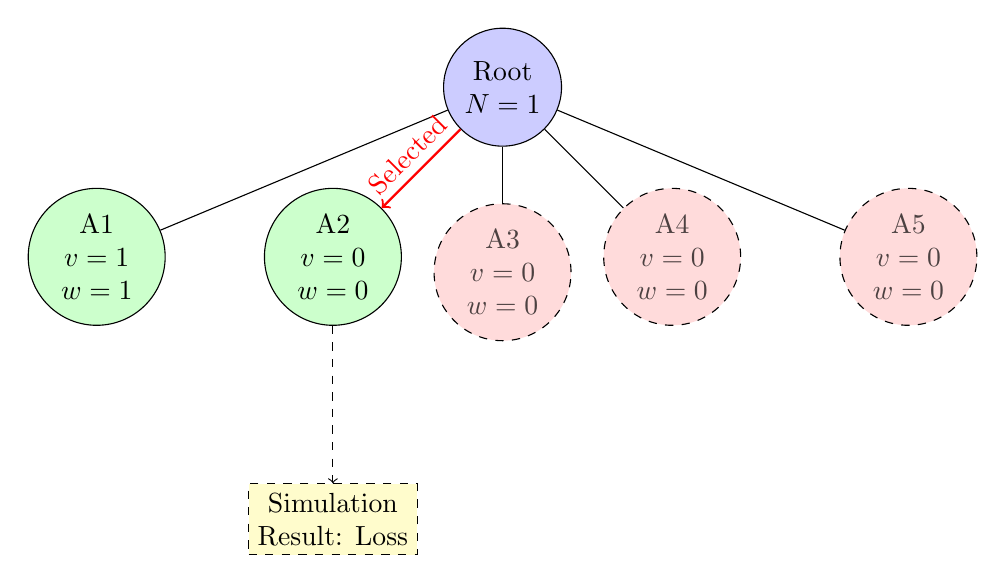
\begin{tikzpicture}[
    node distance=2.35cm,
    treenode/.style={circle, draw, minimum size=1cm, align=center},
    root/.style={treenode, fill=blue!20},
    unvisited/.style={treenode, fill=red!20,
        fill opacity=0.7, % Adjust transparency (0.0 to 1.0)
        draw,              % Ensure a border is drawn
        dashed             % Make the border dashed
        },
    selected/.style={treenode, fill=red!20},
    visited/.style={treenode, fill=green!20},
    simulation/.style={rectangle, draw, dashed, fill=yellow!20, align=center}
]

% Root node
\node[root] (root) {Root \\ $N=1$};

% Previous visited node
\node[visited, below left=1cm and 4cm of root] (a1) {A1 \\ $v=1$ \\ $w=1$};

% A2 is being expanded
\node[visited, below left=1cm and 1cm of root] (a2) {A2 \\ $v=0$ \\ $w=0$};
\node[unvisited, below of=root] (a3) {A3 \\ $v=0$ \\ $w=0$};
\node[unvisited, below right=1cm and 1cm of root] (a4) {A4 \\ $v=0$ \\ $w=0$};
\node[unvisited, below right=1cm and 4cm of root] (a5) {A5 \\ $v=0$ \\ $w=0$};

% Simulation cluster
\node[simulation, below=2cm of a2] (sim2) {Simulation \\ Result: Loss};

% Edges and annotations
\draw (root) -- (a1);
\draw[->, thick, red] (root) -- node[above, sloped] {Selected} (a2);
\draw (root) -- (a3);
\draw (root) -- (a4);
\draw (root) -- (a5);
\draw[dashed, ->] (a2) -- (sim2);

\end{tikzpicture}
\end{center}

\textbf{Backpropagation}: A2 loses $\Rightarrow$ $v=1$, $w=0$, Root $N=2$

\subsection*{Iteration 3: Third Expansion}

Select A3 (remaining unvisited node).

\begin{center}
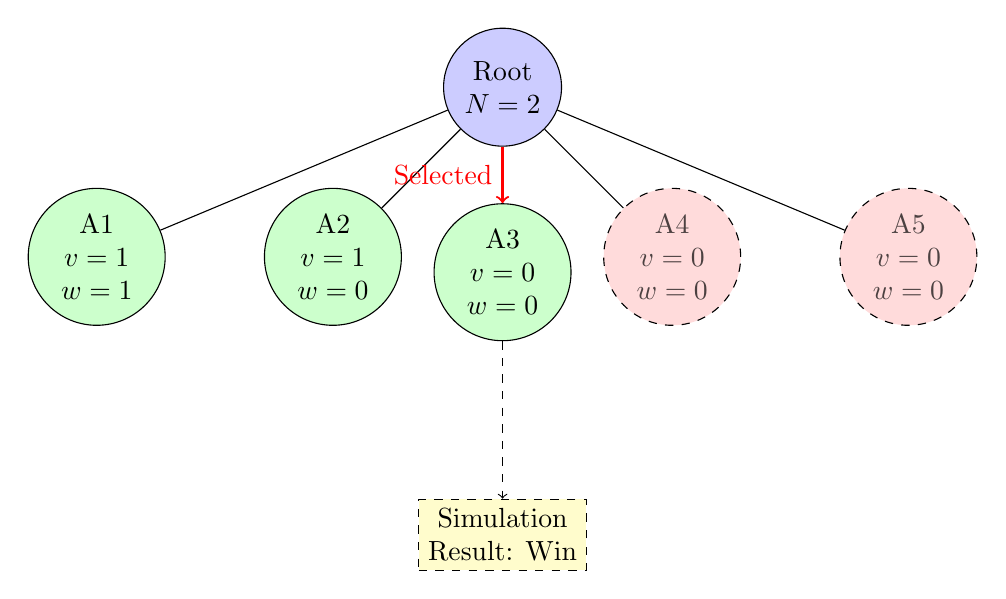
\begin{tikzpicture}[
    node distance=2.35cm,
    treenode/.style={circle, draw, minimum size=1cm, align=center},
    root/.style={treenode, fill=blue!20},
        unvisited/.style={treenode, fill=red!20,
        fill opacity=0.7, % Adjust transparency (0.0 to 1.0)
        draw,              % Ensure a border is drawn
        dashed             % Make the border dashed
        },
    visited/.style={treenode, fill=green!20},
    simulation/.style={rectangle, draw, dashed, fill=yellow!20, align=center}
]

% Root node
\node[root] (root) {Root \\ $N=2$};

% Previous visited nodes
\node[visited, below left=1cm and 4cm of root] (a1) {A1 \\ $v=1$ \\ $w=1$};
\node[visited, below left=1cm and 1cm of root] (a2) {A2 \\ $v=1$ \\ $w=0$};

% A3 is being expanded
\node[visited, below of=root] (a3) {A3 \\ $v=0$ \\ $w=0$};
\node[unvisited, below right=1cm and 1cm of root] (a4) {A4 \\ $v=0$ \\ $w=0$};
\node[unvisited, below right=1cm and 4cm of root] (a5) {A5 \\ $v=0$ \\ $w=0$};

% Simulation cluster
\node[simulation, below=2cm of a3] (sim3) {Simulation \\ Result: Win};

% Edges and annotations
\draw (root) -- (a1);
\draw (root) -- (a2);
\draw[->, thick, red] (root) -- node[left] {Selected} (a3);
\draw (root) -- (a4);
\draw (root) -- (a5);
\draw[dashed, ->] (a3) -- (sim3);

\end{tikzpicture}
\end{center}

\textbf{Backpropagation}: A3 wins $\Rightarrow$ $v=1$, $w=1$, Root $N=3$

\subsection*{Iteration 4: Fourth Expansion}

Select A4 (remaining unvisited node).

\begin{center}
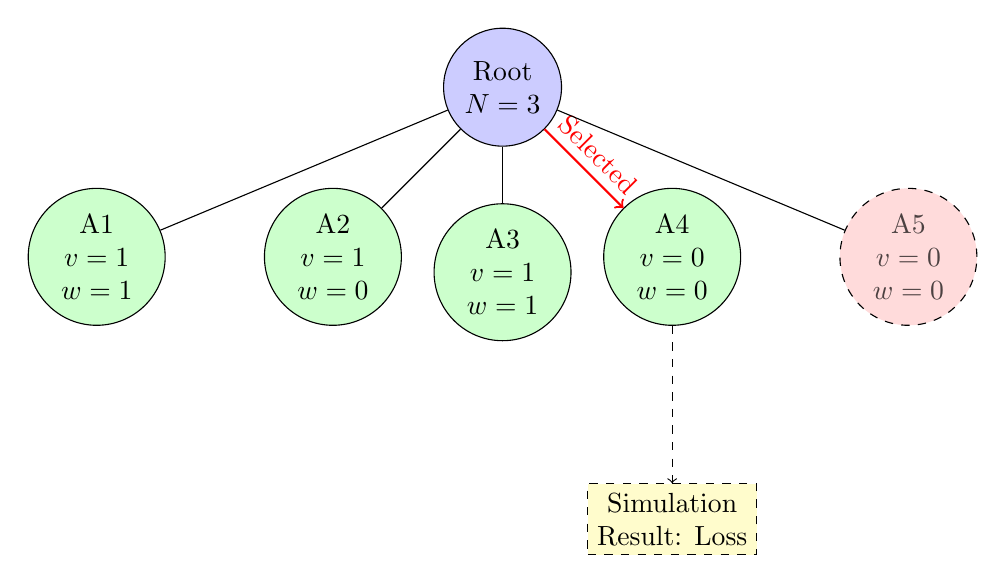
\begin{tikzpicture}[
    node distance=2.35cm,
    treenode/.style={circle, draw, minimum size=1cm, align=center},
    root/.style={treenode, fill=blue!20},
        unvisited/.style={treenode, fill=red!20,
        fill opacity=0.7, % Adjust transparency (0.0 to 1.0)
        draw,              % Ensure a border is drawn
        dashed             % Make the border dashed
        },
    visited/.style={treenode, fill=green!20},
    simulation/.style={rectangle, draw, dashed, fill=yellow!20, align=center}
]

% Root node
\node[root] (root) {Root \\ $N=3$};

% Previous visited nodes
\node[visited, below left=1cm and 4cm of root] (a1) {A1 \\ $v=1$ \\ $w=1$};
\node[visited, below left=1cm and 1cm of root] (a2) {A2 \\ $v=1$ \\ $w=0$};
\node[visited, below of=root] (a3) {A3 \\ $v=1$ \\ $w=1$};

% A4 is being expanded
\node[visited, below right=1cm and 1cm of root] (a4) {A4 \\ $v=0$ \\ $w=0$};
\node[unvisited, below right=1cm and 4cm of root] (a5) {A5 \\ $v=0$ \\ $w=0$};

% Simulation cluster
\node[simulation, below=2cm of a4] (sim4) {Simulation \\ Result: Loss};

% Edges and annotations
\draw (root) -- (a1);
\draw (root) -- (a2);
\draw (root) -- (a3);
\draw[->, thick, red] (root) -- node[above, sloped] {Selected} (a4);
\draw (root) -- (a5);
\draw[dashed, ->] (a4) -- (sim4);

\end{tikzpicture}
\end{center}

\textbf{Backpropagation}: A4 loses $\Rightarrow$ $v=1$, $w=0$, Root $N=4$

\subsection*{Iteration 5: Final Initial Expansion}

Select A5 (last unvisited node).

\begin{center}
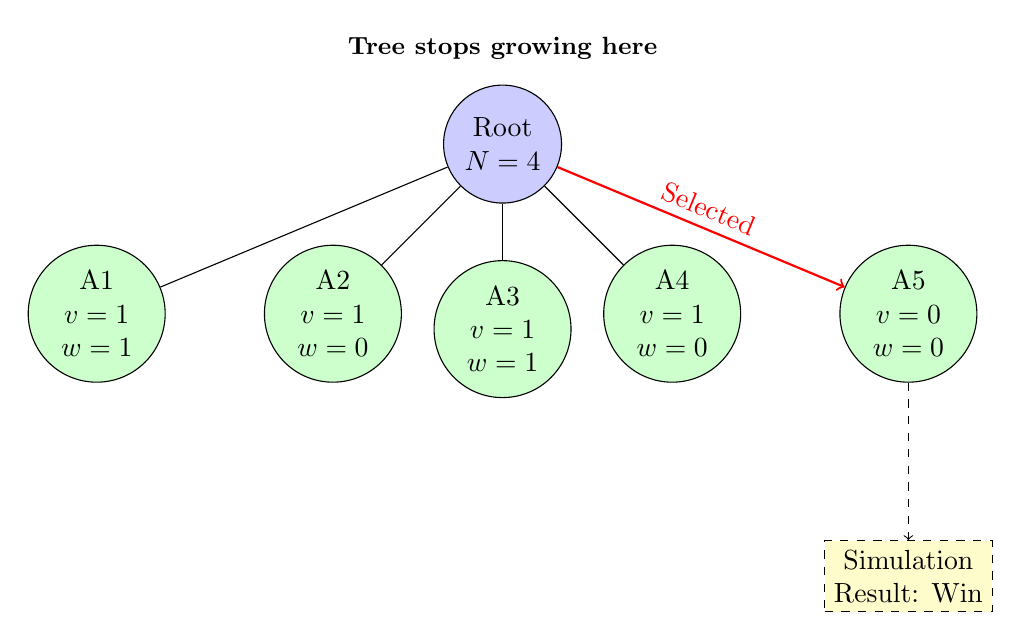
\begin{tikzpicture}[
    node distance=2.35cm,
    treenode/.style={circle, draw, minimum size=1cm, align=center},
    root/.style={treenode, fill=blue!20},
        unvisited/.style={treenode, fill=red!20,
        fill opacity=0.7, % Adjust transparency (0.0 to 1.0)
        draw,              % Ensure a border is drawn
        dashed             % Make the border dashed
        },
    visited/.style={treenode, fill=green!20},
    simulation/.style={rectangle, draw, dashed, fill=yellow!20, align=center}
]

% Root node
\node[root] (root) {Root \\ $N=4$};

% All nodes now visited
\node[visited, below left=1cm and 4cm of root] (a1) {A1 \\ $v=1$ \\ $w=1$};
\node[visited, below left=1cm and 1cm of root] (a2) {A2 \\ $v=1$ \\ $w=0$};
\node[visited, below of=root] (a3) {A3 \\ $v=1$ \\ $w=1$};
\node[visited, below right=1cm and 1cm of root] (a4) {A4 \\ $v=1$ \\ $w=0$};

% A5 is being expanded (last one)
\node[visited, below right=1cm and 4cm of root] (a5) {A5 \\ $v=0$ \\ $w=0$};

% Simulation cluster
\node[simulation, below=2cm of a5] (sim5) {Simulation \\ Result: Win};

% Edges and annotations
\draw (root) -- (a1);
\draw (root) -- (a2);
\draw (root) -- (a3);
\draw (root) -- (a4);
\draw[->, thick, red] (root) -- node[above, sloped] {Selected} (a5);
\draw[dashed, ->] (a5) -- (sim5);

\node[above=0.2cm of root] {\small\textbf{Tree stops growing here}};

\end{tikzpicture}
\end{center}

\textbf{Backpropagation}: A5 wins $\Rightarrow$ $v=1$, $w=1$, Root $N=5$

\subsection*{Iteration 6: First UCB1 Selection}

Now all nodes have been visited. Calculate UCB1 ($c = \sqrt{2}$):

\begin{align*}
\text{UCB1}(A1) &= \frac{1}{1} + \sqrt{2} \sqrt{\frac{\ln 5}{1}} = 1 + 1.87 = 2.87 \\
\text{UCB1}(A2) &= \frac{0}{1} + \sqrt{2} \sqrt{\frac{\ln 5}{1}} = 0 + 1.87 = 1.87 \\
\text{UCB1}(A3) &= \frac{1}{1} + \sqrt{2} \sqrt{\frac{\ln 5}{1}} = 1 + 1.87 = 2.87 \\
\text{UCB1}(A4) &= \frac{0}{1} + \sqrt{2} \sqrt{\frac{\ln 5}{1}} = 0 + 1.87 = 1.87 \\
\text{UCB1}(A5) &= \frac{1}{1} + \sqrt{2} \sqrt{\frac{\ln 5}{1}} = 1 + 1.87 = 2.87
\end{align*}

Tie between A1, A3, A5. Randomly select A1.

\begin{center}
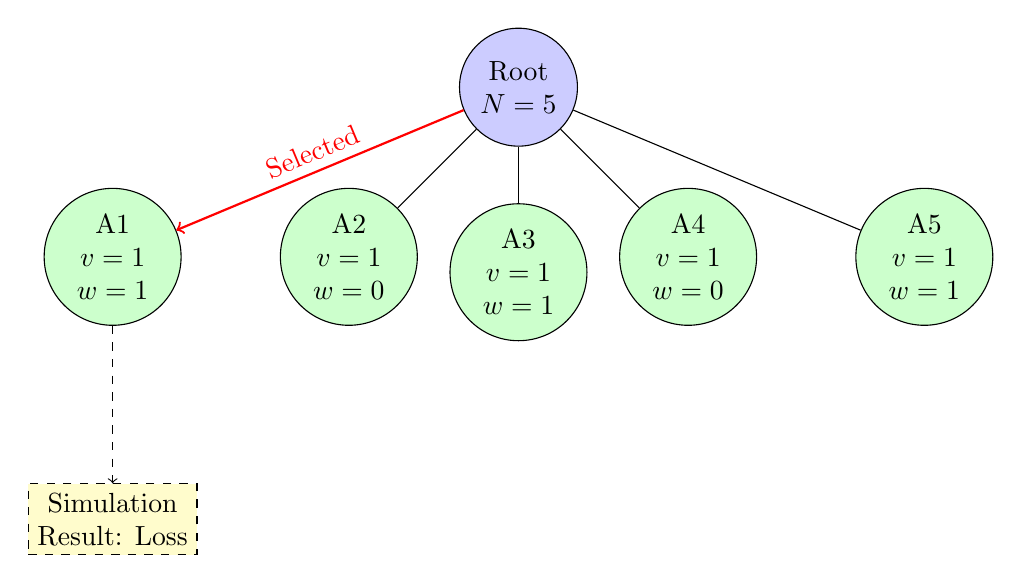
\begin{tikzpicture}[
    node distance=2.35cm,
    treenode/.style={circle, draw, minimum size=1cm, align=center},
    root/.style={treenode, fill=blue!20},
    visited/.style={treenode, fill=green!20},
    simulation/.style={rectangle, draw, dashed, fill=yellow!20, align=center}
]

% Root node
\node[root] (root) {Root \\ $N=5$};

% All nodes visited
\node[visited, below left=1cm and 4cm of root] (a1) {A1 \\ $v=1$ \\ $w=1$};
\node[visited, below left=1cm and 1cm of root] (a2) {A2 \\ $v=1$ \\ $w=0$};
\node[visited, below of=root] (a3) {A3 \\ $v=1$ \\ $w=1$};
\node[visited, below right=1cm and 1cm of root] (a4) {A4 \\ $v=1$ \\ $w=0$};
\node[visited, below right=1cm and 4cm of root] (a5) {A5 \\ $v=1$ \\ $w=1$};

% Simulation cluster
\node[simulation, below=2cm of a1] (sim6) {Simulation \\ Result: Loss};

% Edges and annotations
\draw[->, thick, red] (root) -- node[above, sloped] {Selected} (a1);
\draw (root) -- (a2);
\draw (root) -- (a3);
\draw (root) -- (a4);
\draw (root) -- (a5);
\draw[dashed, ->] (a1) -- (sim6);

\end{tikzpicture}
\end{center}

\textbf{Backpropagation}: 
Only updates selected node $A_1$: $v=2$, $w=1$, Root $N=6$

\section*{Final Tree State}

After many iterations, the tree might look like:

\begin{center}
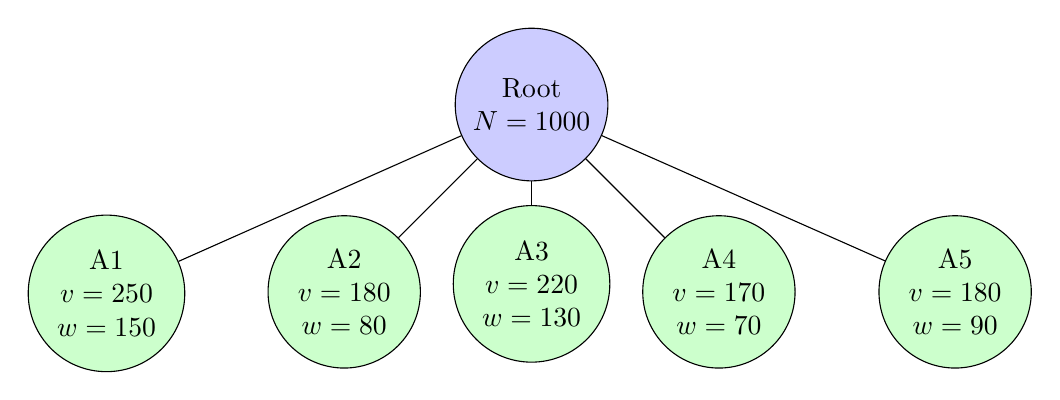
\begin{tikzpicture}[
    node distance=2.35cm,
    treenode/.style={circle, draw, minimum size=1cm, align=center},
    root/.style={treenode, fill=blue!20},
    visited/.style={treenode, fill=green!20, align=center}
]

% Root node
\node[root] (root) {Root \\ $N=1000$};

% Final statistics
\node[visited, below left=1cm and 4cm of root] (a1) {A1 \\ $v=250$ \\ $w=150$};
\node[visited, below left=1cm and 1cm of root] (a2) {A2 \\ $v=180$ \\ $w=80$};
\node[visited, below=0.3cm of root] (a3) {A3 \\ $v=220$ \\ $w=130$};
\node[visited, below right=1cm and 1cm of root] (a4) {A4 \\ $v=170$ \\ $w=70$};
\node[visited, below right=1cm and 4cm of root] (a5) {A5 \\ $v=180$ \\ $w=90$};

% Edges
\draw (root) -- (a1);
\draw (root) -- (a2);
\draw (root) -- (a3);
\draw (root) -- (a4);
\draw (root) -- (a5);

\end{tikzpicture}
\end{center}

\textbf{Final Decision}: Choose move with highest win rate: A1 ($150/250 = 60\%$)

\end{document}